\subsection{Berechnung: Analytischen Lösung der Modellierung}\label{Lösung}
In diesem Abschnitt werden die Gleichungen \ref{eq:34}, \ref{eq:35} und \ref{eq:36} herlgeleitet:
\begin{itemize}
	\item Aus Gleichung \ref{eq:11} und \ref{eq:22} ergibt sich:
	\begin{equation}\label{eq:164}
		R_{4}=0
	\end{equation}
	\item Aus Gleichung \ref{eq:9} und \ref{eq:23} ergibt sich:
	\begin{equation}\label{eq:165}
		R_{2}=0
	\end{equation}
	\item Aus Gleichung \ref{eq:18} und \ref{eq:33} ergibt sich:
	\begin{equation}\label{eq:166}
		R_{9}=-F
	\end{equation}
	\item Aus Gleichung \ref{eq:13}, \ref{eq:18}, \ref{eq:33} und \ref{eq:166} ergibt sich:
	\begin{equation}\label{eq:167}
		R_{5}=-F_{pruef}-F_{Q}
	\end{equation}
	\item Aus Gleichung \ref{eq:19} , \ref{eq:32} und \ref{eq:166} ergibt sich:
	\begin{equation}\label{eq:168}
		R_{10}=F_{pruef}\cdot (l_{1}+l_{2}+l_{3})
	\end{equation}
	\item Aus Gleichung \ref{eq:14}, \ref{eq:19}, \ref{eq:30}, \ref{eq:166}, \ref{eq:167} und \ref{eq:168} ergibt sich:
	\begin{equation}\label{eq:169}
		R_{6}=F_{pruef}\cdot (l_{1}+l_{2}+l_{3}) + F_{Q}\cdot (l_{1}+l_{2})
	\end{equation}
	\item Aus Gleichung \ref{eq:9}, \ref{eq:14}, \ref{eq:27}, \ref{eq:167} und \ref{eq:169} ergibt sich:
	\begin{equation}\label{eq:170}
		R_{1}=F_{pruef}\cdot\frac{l_{2}+l_{3}}{l_{1}} + F_{Q}\cdot\frac{l_{2}}{l_{1}}
	\end{equation}
	\item Aus Gleichung \ref{eq:11}, \ref{eq:24} und \ref{eq:170} ergibt sich:
	\begin{equation}\label{eq:171}
		R_{3}=-\frac{1}{6}\cdot F_{pruef}\cdot (l_{2}+l_{3})\cdot l_{1} - \frac{1}{6}\cdot F_{Q}\cdot l_{2}\cdot l_{1}
	\end{equation}
	\item Aus Gleichung \ref{eq:10}, \ref{eq:15}, \ref{eq:26}, \ref{eq:167}, \ref{eq:169}, \ref{eq:170} und \ref{eq:171} ergibt sich:
	\begin{equation}\label{eq:172}
		R_{7}=F_{pruef}\cdot \Bigl(-\frac{1}{2} l_{1}^{2}-\frac{2}{3} l_{1}l{2}-\frac{2}{3} l_{1}l{3}\Bigr) + F_{Q}\cdot \Bigl(-\frac{1}{2} l_{1}^{2}-\frac{2}{3} l_{1}l{2}\Bigr)
	\end{equation}
	\item Aus Gleichung \ref{eq:16}, \ref{eq:25}, \ref{eq:167}, \ref{eq:169} und \ref{eq:172} ergibt sich:
	\begin{equation}\label{eq:173}
		R_{8}=F_{pruef}\cdot \Bigl(\frac{1}{6} l_{1}^{3}+\frac{1}{6} l_{1}^{2}l{2}+\frac{1}{6} l_{1}^{2}l{3}\Bigr) + F_{Q}\cdot \Bigl(\frac{1}{6} l_{1}^{3}+\frac{1}{6} l_{1}^{2}l{2}\Bigr)
	\end{equation}
	\item Aus Gleichung \ref{eq:15}, \ref{eq:20}, \ref{eq:29}, \ref{eq:166}, \ref{eq:167}, \ref{eq:168}, \ref{eq:169} und \ref{eq:172} ergibt sich:
	\begin{equation}\label{eq:174}
		R_{11}=F_{pruef}\cdot \Bigl(-\frac{1}{2} l_{1}^{2}-\frac{2}{3} l_{1}l{2}-\frac{2}{3} l_{1}l{3}\Bigr) + F_{Q}\cdot \Bigl(\frac{1}{2} l_{1}^{2}+\frac{1}{3} l_{1}l{2}\Bigr)
	\end{equation}
	\item Aus Gleichung \ref{eq:16}, \ref{eq:21}, \ref{eq:28}, \ref{eq:166}, \ref{eq:167}, \ref{eq:168}, \ref{eq:169}, \ref{eq:172}, \ref{eq:173} und \ref{eq:174} ergibt sich:
	\begin{equation}\label{eq:175}
		R_{12}=F_{pruef}\cdot \Bigl(\frac{1}{6} l_{1}^{3}+\frac{1}{6} l_{1}^{2}l{2}+\frac{1}{6} l_{1}^{2}l{3}\Bigr) + F_{Q}\cdot \Bigl(\frac{1}{6} l_{2}^{3}-\frac{1}{3} l_{1}^{2}l{2}-\frac{1}{2} l_{2}^{2}l{1}\Bigr)
	\end{equation}
	\item Nun können die Gleichungen \ref{eq:166}, \ref{eq:167}, und \ref{eq:170} in folgende Gleichung eingesetzt werden, sodass sich Gleichung \ref{eq:34} ergibt:
	\begin{equation}
		Q(y,F_{pruef},F_{Q},EI_{x})=\left\{\begin{array}{ll}
			-R_{1}&,y\epsilon (0,l_{1})\\
			-R_{5}&,y\epsilon (l_{1}, l_{1}+l_{2})\\
			-R_{9}&,y\epsilon (l_{1}+l_{2}, l_{1}+l_{2}+l_{3})
		\end{array}\right.
	\end{equation}
	\item Nun können die Gleichungen \ref{eq:165}, \ref{eq:166}, \ref{eq:167}, \ref{eq:168}, \ref{eq:169} und \ref{eq:170} in folgende Gleichung eingesetzt werden, sodass sich Gleichung \ref{eq:35} ergibt:
	\begin{equation}
		M(y,F_{pruef},F_{Q},EI_{x})=\left\{\begin{array}{ll}
			-R_{1}\cdot y - R_{2}&,y\epsilon (0,l_{1})\\
			-R_{5}\cdot y - R_{6}&,y\epsilon (l_{1}, l_{1}+l_{2})\\
			-R_{9}\cdot y - R_{10}&,y\epsilon (l_{1}+l_{2}, l_{1}+l_{2}+l_{3})
		\end{array}\right.
	\end{equation}
	\item Nun können die Gleichungen  \ref{eq:164}, \ref{eq:165}, \ref{eq:166}, \ref{eq:167}, \ref{eq:168}, \ref{eq:169}, \ref{eq:170},  \ref{eq:171},  \ref{eq:172},  \ref{eq:172},  \ref{eq:174} und  \ref{eq:175} in folgende Gleichung eingesetzt werden, sodass sich Gleichung \ref{eq:36} ergibt:
	\begin{equation}
		w(y,F_{pruef},F_{Q},EI_{x})=\left\{\begin{array}{ll}
			\frac{1}{EI}\cdot\Bigl(\frac{R_{1}\cdot y^{3}}{6}+\frac{R_{2}\cdot y^{2}}{2}+R_{3}\cdot y +R_{4}\Bigr)&,y\epsilon (0,l_{1})\\
			\frac{1}{EI}\cdot\Bigl(\frac{R_{5}\cdot y^{3}}{6}+\frac{R_{6}\cdot y^{2}}{2}+R_{7}\cdot y +R_{8}\Bigr)&,y\epsilon (l_{1}, l_{1}+l_{2})\\
			\frac{1}{EI}\cdot\Bigl(\frac{R_{9}\cdot y^{3}}{6}+\frac{R_{10}\cdot y^{2}}{2}+R_{11}\cdot y +R_{12}\Bigr)&,y\epsilon (l_{1}+l_{2}, l_{1}+l_{2}+l_{3})
		\end{array}\right.
	\end{equation}
\end{itemize}
\newpage
\subsection{Abbildungen}\label{Abbildungen}
\begin{figure}[h]
	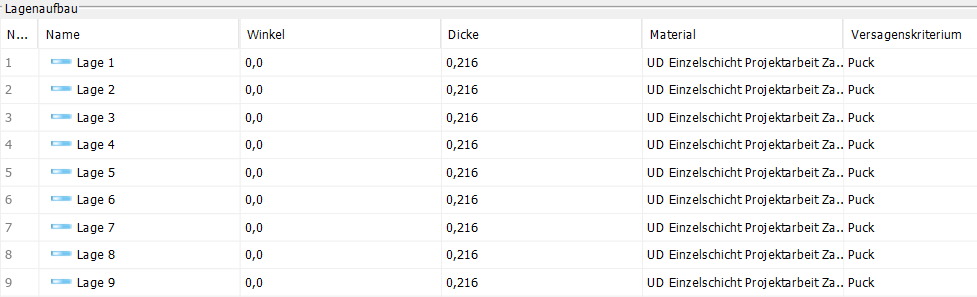
\includegraphics[width=1.0\textwidth]{Bilder/Lagenaufbau Holmgurte.png}
	\caption{Lagenaufbau Holmgurte}
	\label{fig:Lagenaufbau Holmgurte}
\end{figure}
\begin{figure}[h]
	\includegraphics[width=1.0\textwidth]{Bilder/Lagenaufbau Steg dünn.png}
	\caption{Lagenaufbau Steg Bereich $III$}
	\label{fig:Lagenaufbau Steg dünn}
\end{figure}
\begin{figure}[h]
	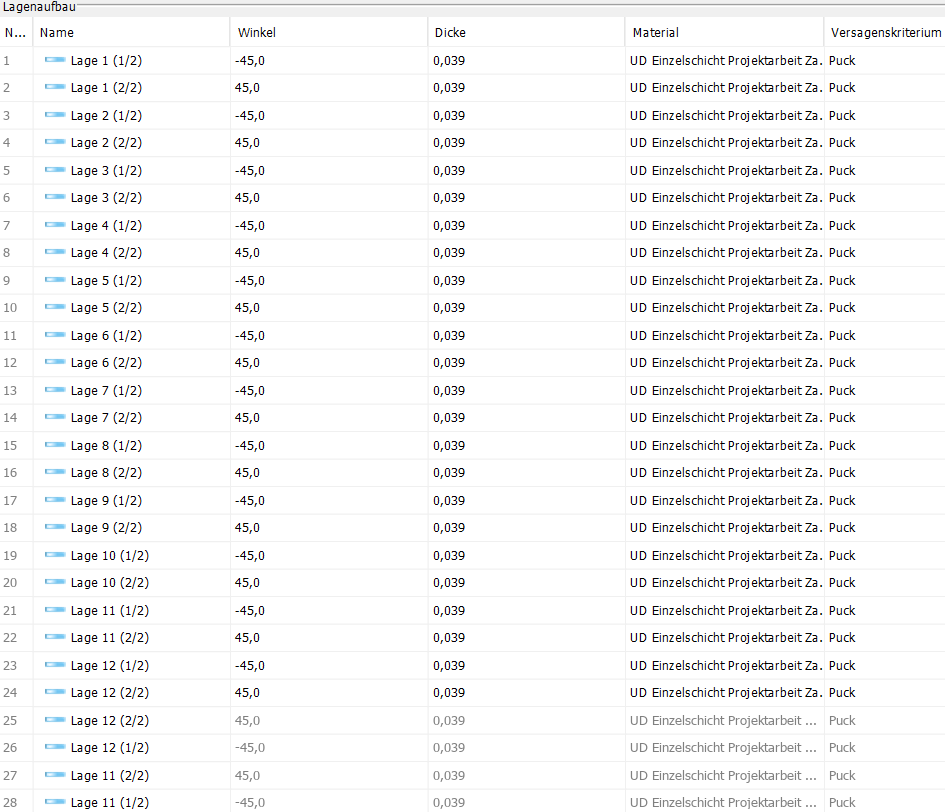
\includegraphics[width=1.0\textwidth]{Bilder/Lagenaufbau Steg dick.png}
	\caption{Lagenaufbau Steg Bereich $I$\&$II$}
	\label{fig:Lagenaufbau Steg dick}
\end{figure}
\begin{figure}[h]
	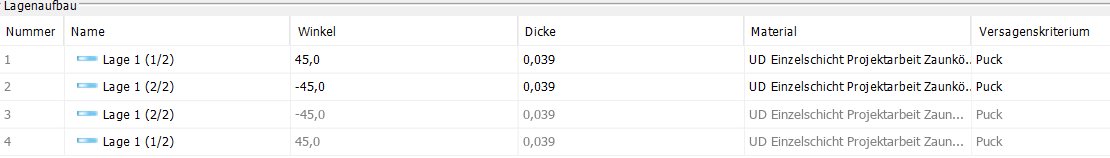
\includegraphics[width=1.0\textwidth]{Bilder/Lagenaufbau Haut.png}
	\caption{Lagenaufbau Flügelschale}
	\label{fig:Lagenaufbau Haut}
\end{figure}
\begin{figure}[h]
	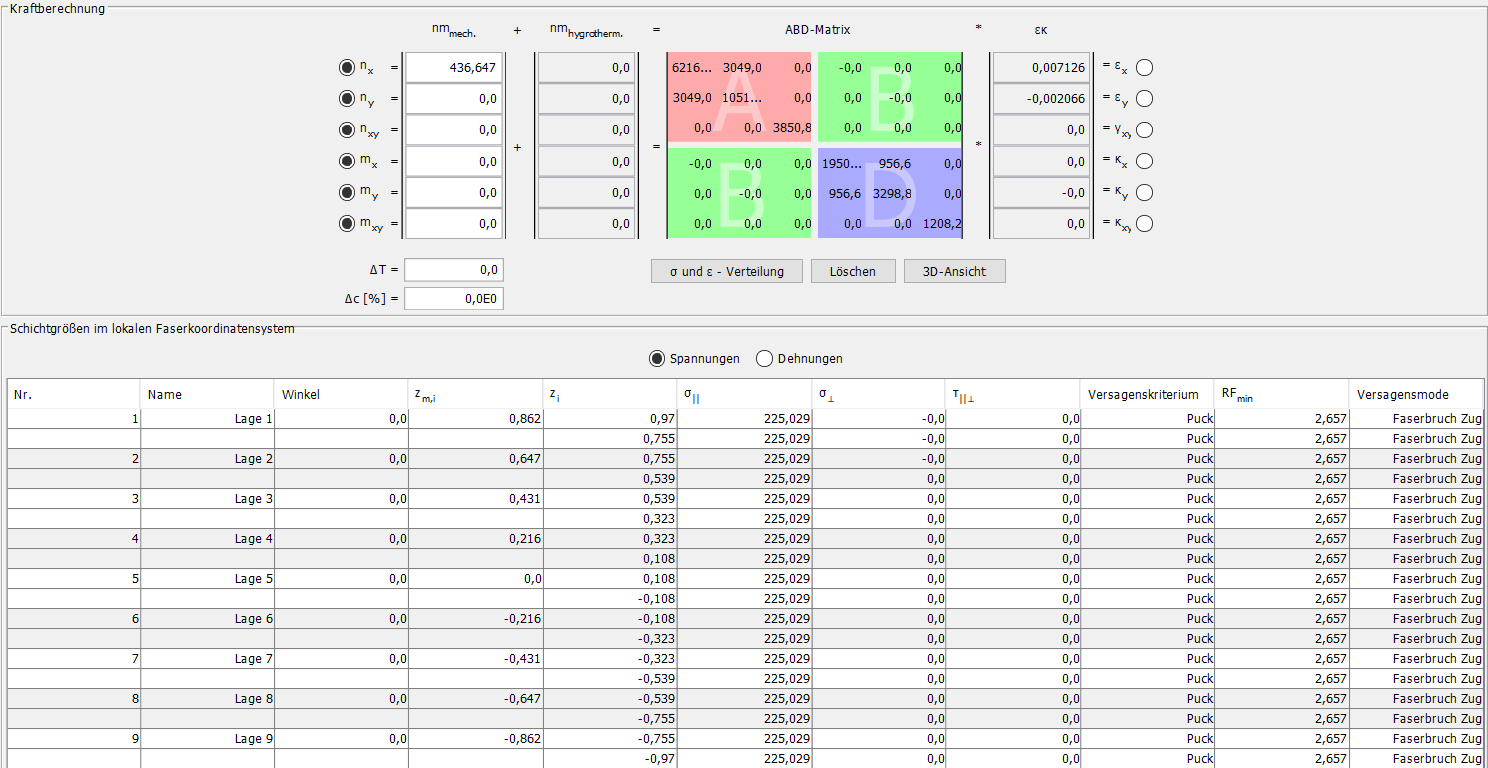
\includegraphics[width=1.0\textwidth]{Bilder/Berechnung Holmgurte.png}
	\caption{Berechnung Holmgurte}
	\label{fig:Berechnung Holmgurte}
\end{figure}
\begin{figure}[h]
	\includegraphics[width=1.0\textwidth]{Bilder/Berechnung Steg dünn.png}
	\caption{Berechnung Steg Bereich $III$}
	\label{fig:Berechnung Steg dünn}
\end{figure}
\begin{figure}[h]
	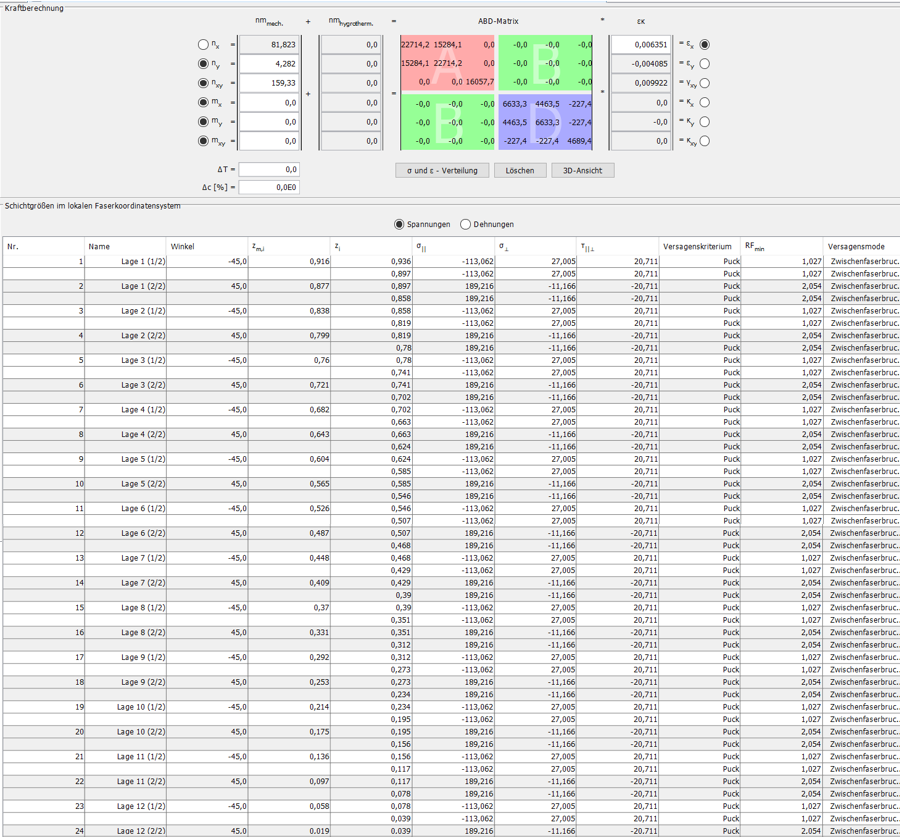
\includegraphics[width=1.0\textwidth]{Bilder/Berechnung Steg dick.png}
	\caption{Berechnung Steg Bereich $I$\&$II$}
	\label{fig:Berechnung Steg dick}
\end{figure}
\begin{figure}[h]
	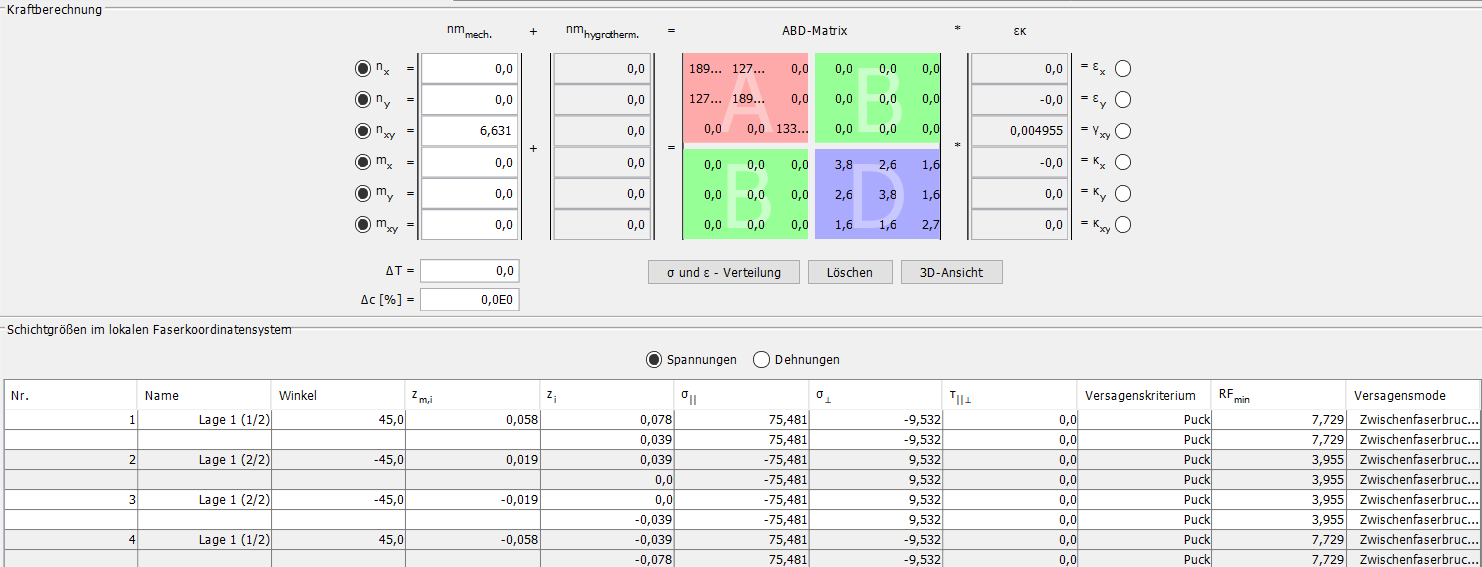
\includegraphics[width=1.0\textwidth]{Bilder/Berechnung Haut.png}
	\caption{Berechnung Flügelschale}
	\label{fig:Berechnung Haut}
\end{figure}
\begin{figure}[h]
	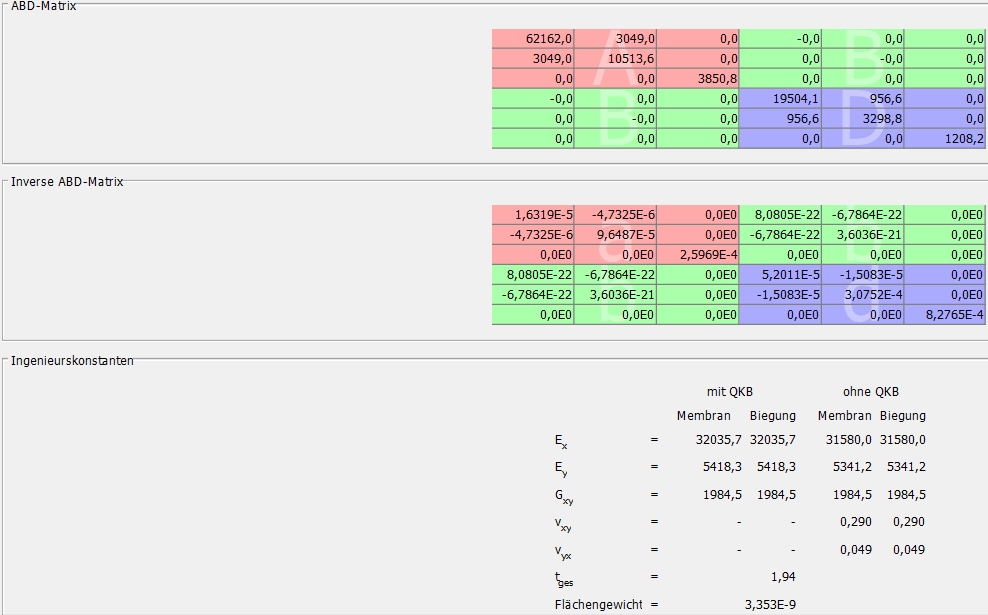
\includegraphics[width=1.0\textwidth]{Bilder/Konstanten Holmgurte.png}
	\caption{Ingenieurskonstanten Holmgurte}
	\label{fig:Ingenieurskonstanten Holmgurte}
\end{figure}
\begin{figure}[h]
	\includegraphics[width=1.0\textwidth]{Bilder/Konstanten Steg dünn.png}
	\caption{BerechnIngenieurskonstantenung Steg Bereich $III$}
	\label{fig:Ingenieurskonstanten Steg dünn}
\end{figure}
\begin{figure}[h]
	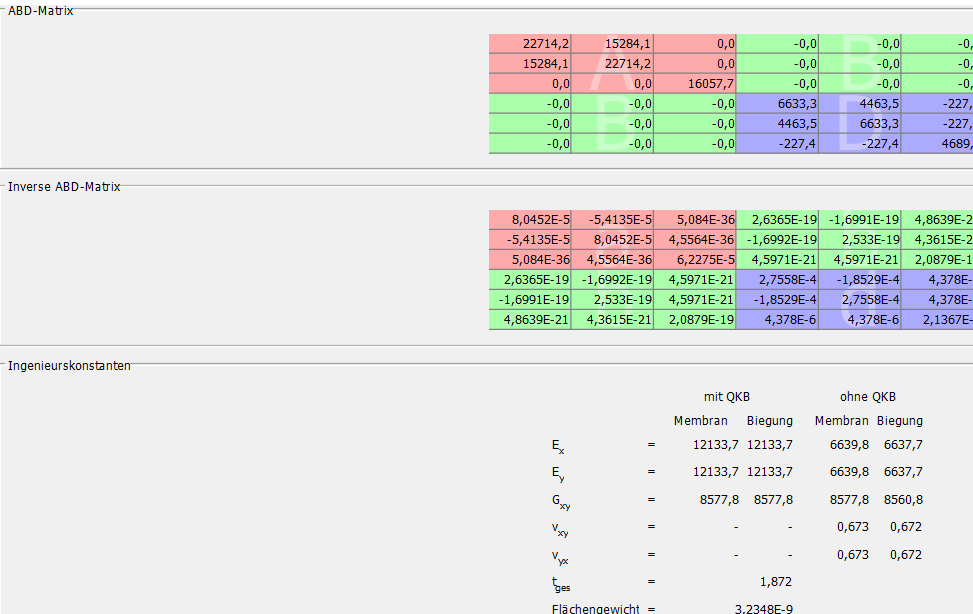
\includegraphics[width=1.0\textwidth]{Bilder/Konstanten Steg dick.png}
	\caption{BerechnIngenieurskonstantenung Steg Bereich $I\&II$}
	\label{fig:Ingenieurskonstanten Steg dick}
\end{figure}
\begin{figure}[h]
	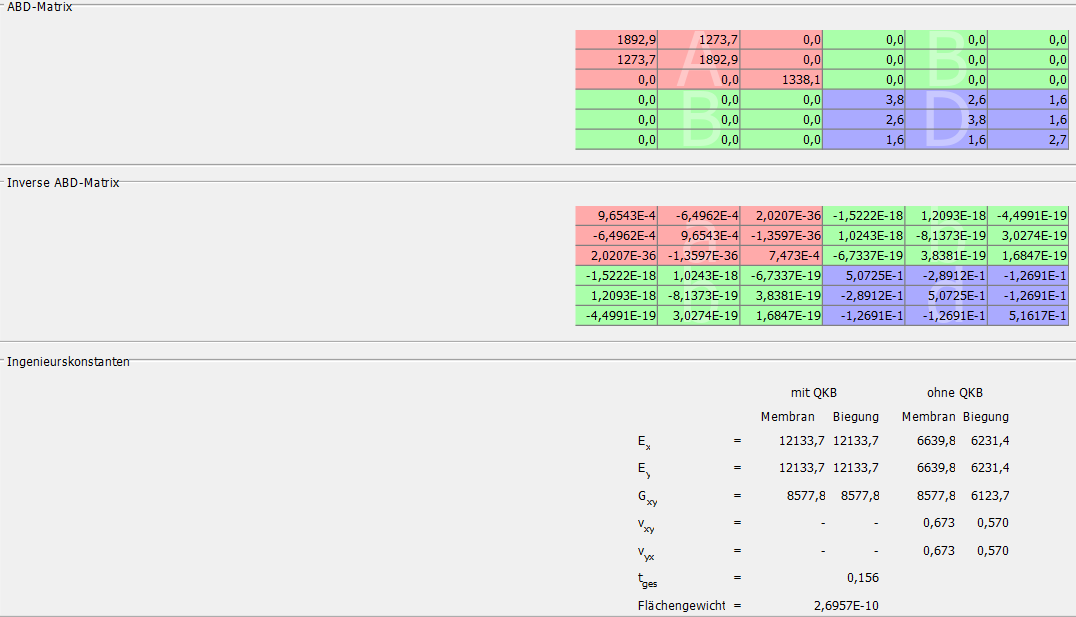
\includegraphics[width=1.0\textwidth]{Bilder/Konstanten Haut.png}
	\caption{Ingenieurskonstanten Flügelschale}
	\label{fig:Ingenieurskonstanten Haut}
\end{figure}
\begin{figure}[h]
	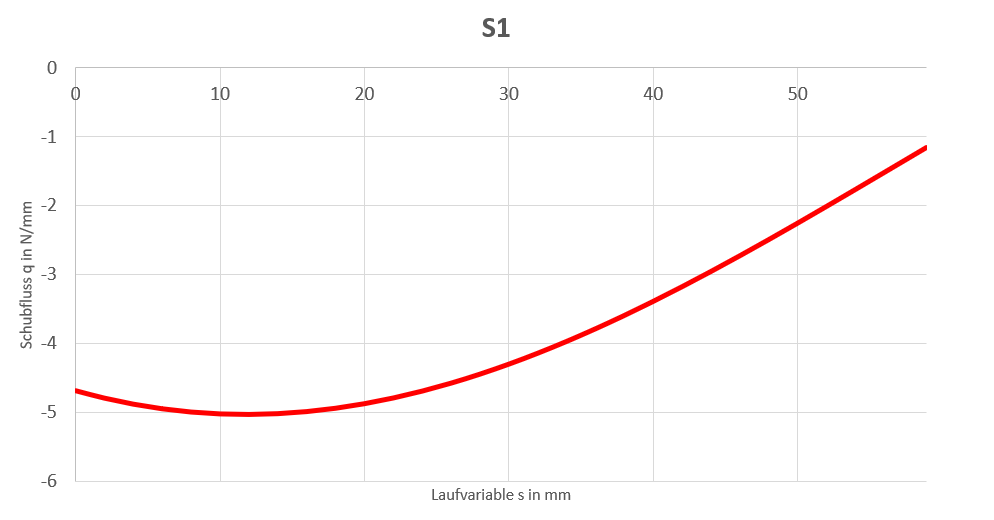
\includegraphics[width=1.0\textwidth]{Bilder/S1.png}
	\caption{Schubfluss Bereich 1}
	\label{fig:S1}
\end{figure}
\begin{figure}[h]
	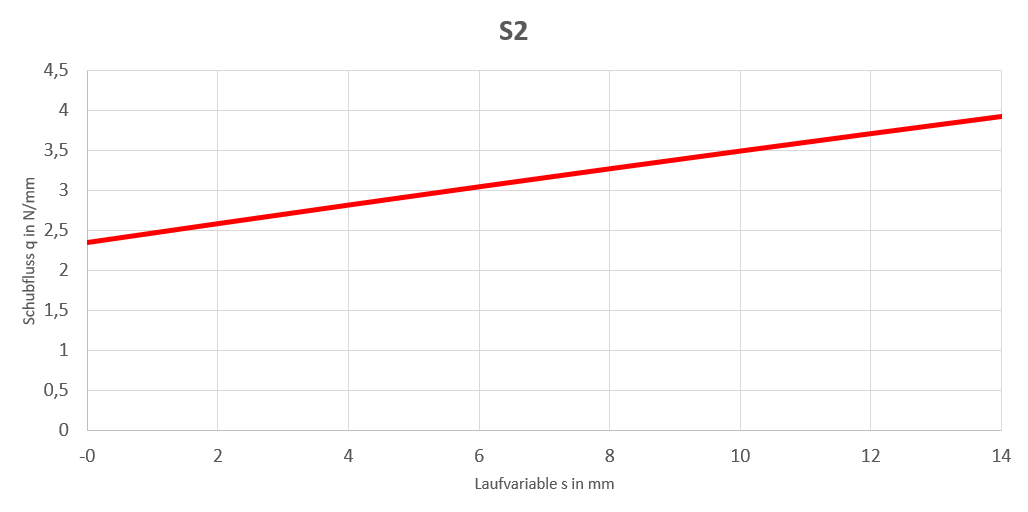
\includegraphics[width=1.0\textwidth]{Bilder/S2.png}
	\caption{Schubfluss Bereich 2}
\end{figure}
\begin{figure}[h]
	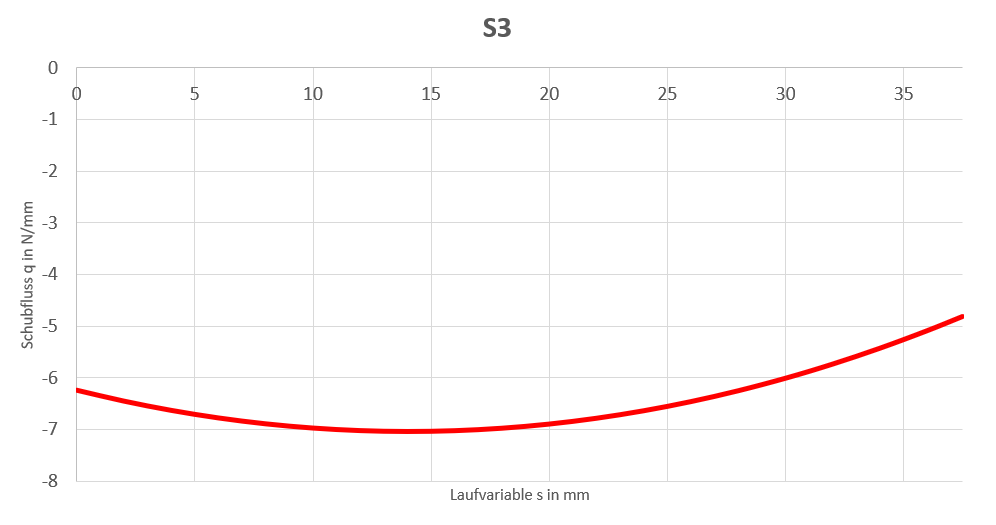
\includegraphics[width=1.0\textwidth]{Bilder/S3.png}
	\caption{Schubfluss Bereich 3}
\end{figure}
\begin{figure}[h]
	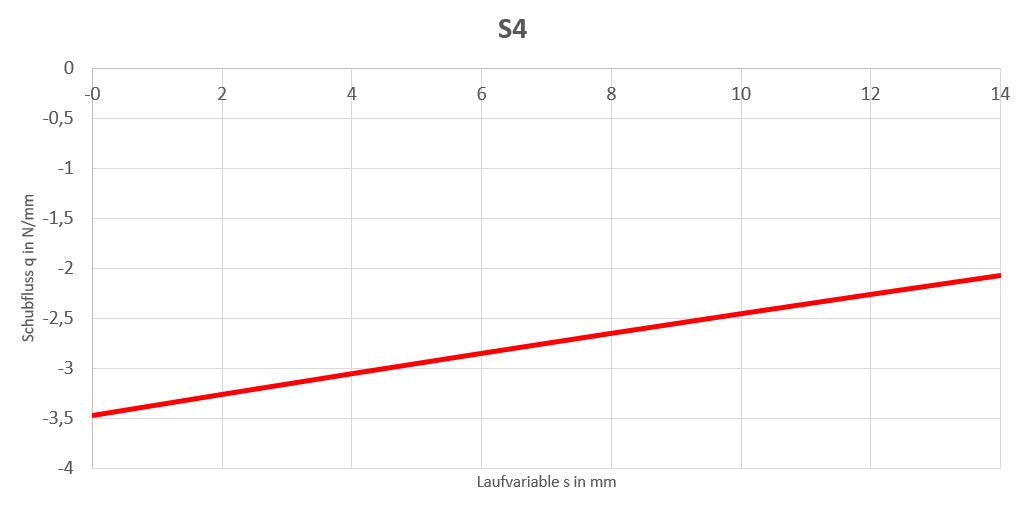
\includegraphics[width=1.0\textwidth]{Bilder/S4.png}
	\caption{Schubfluss Bereich 4}
	\label{fig:S4}
\end{figure}
\begin{figure}[h]
	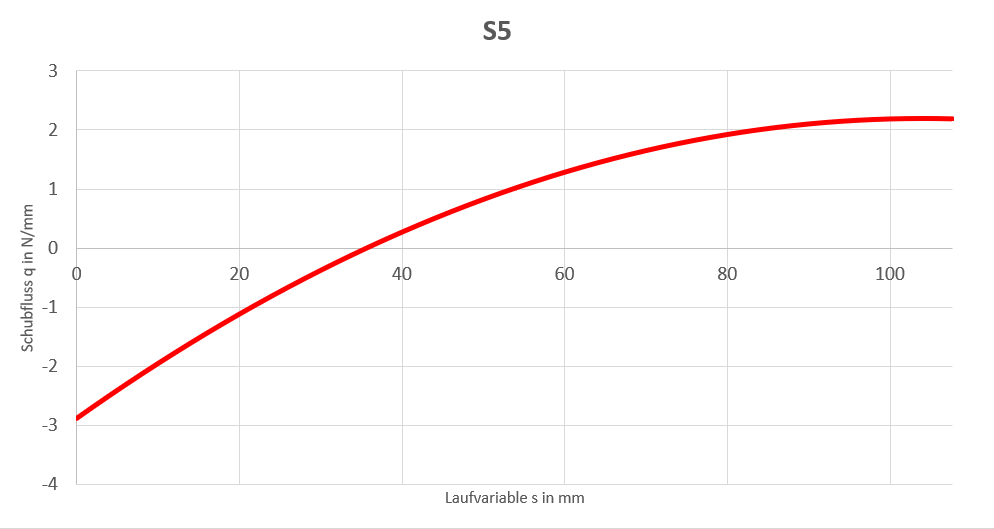
\includegraphics[width=1.0\textwidth]{Bilder/S5.png}
	\caption{Schubfluss Bereich 5}
\end{figure}
\begin{figure}[h]
	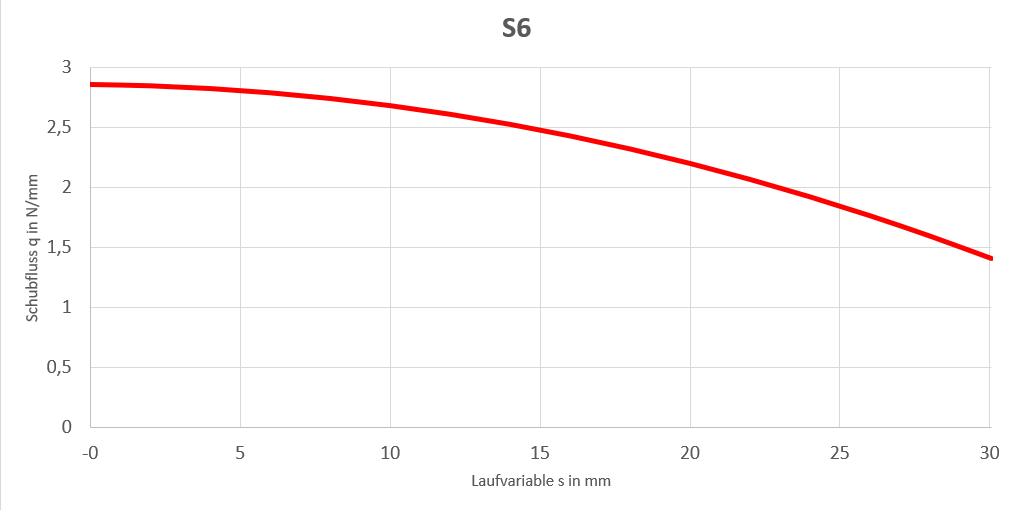
\includegraphics[width=1.0\textwidth]{Bilder/S6.png}
	\caption{Schubfluss Bereich 6}
\end{figure}
\begin{figure}[h]
	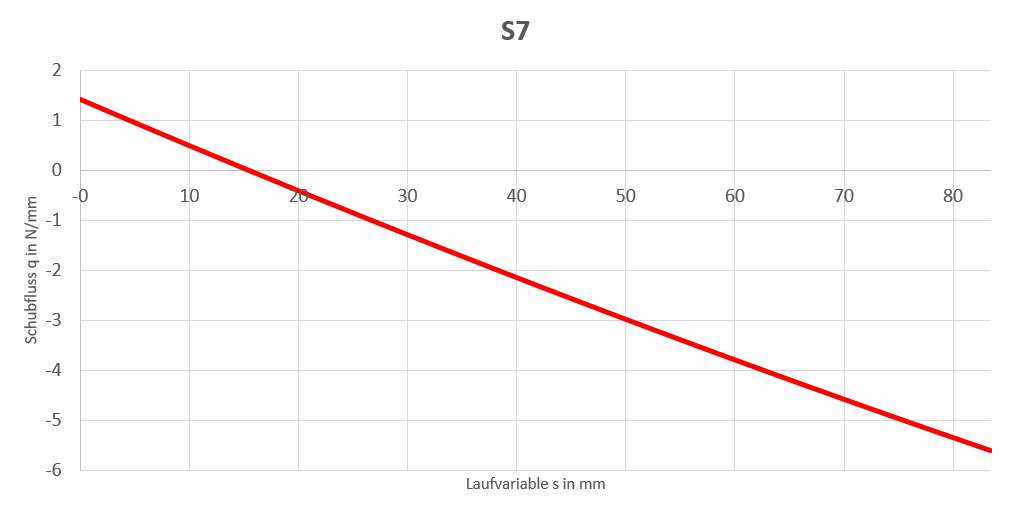
\includegraphics[width=1.0\textwidth]{Bilder/S7.png}
	\caption{Schubfluss Bereich 7}
\end{figure}
\begin{figure}[h]
	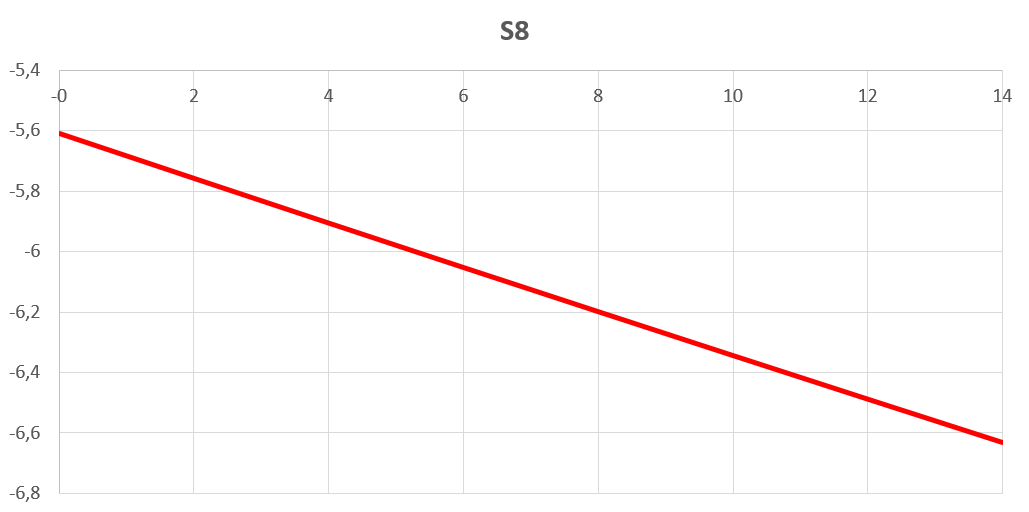
\includegraphics[width=1.0\textwidth]{Bilder/S8.png}
	\caption{Schubfluss Bereich 8}
\end{figure}
\begin{figure}[h]
	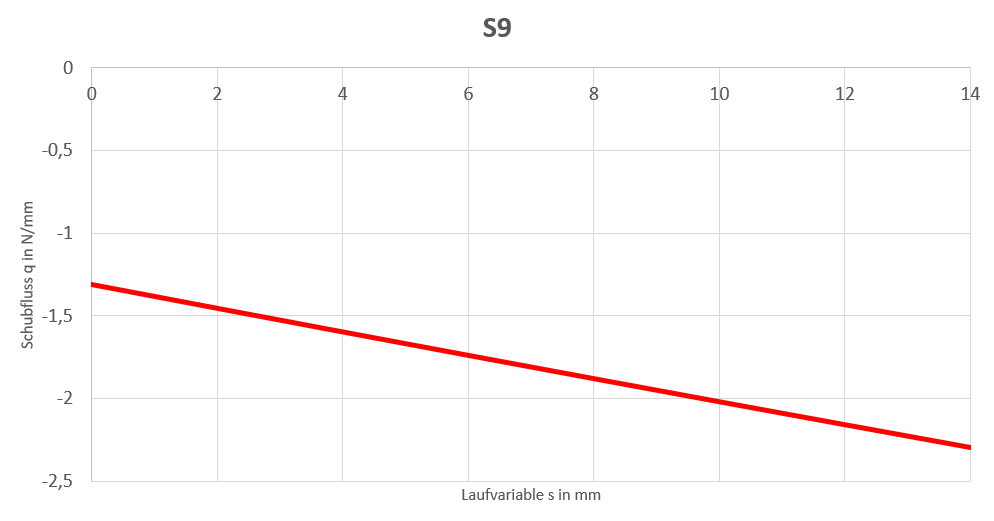
\includegraphics[width=1.0\textwidth]{Bilder/S9.png}
	\caption{Schubfluss Bereich 9}
\end{figure}
\begin{figure}[h]
	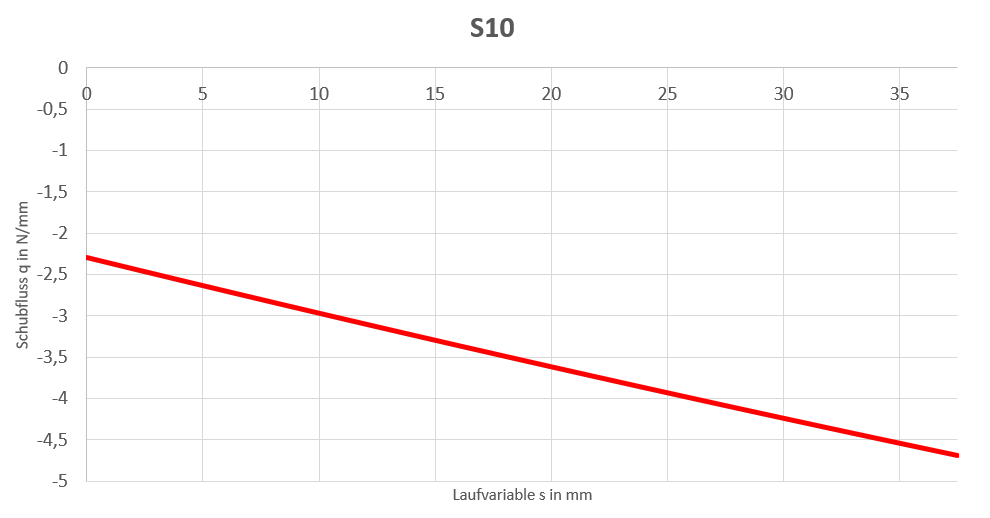
\includegraphics[width=1.0\textwidth]{Bilder/S10.png}
	\caption{Schubfluss Bereich 10}
	\label{fig:S10}
\end{figure}
\newpage
%Technische Zeichnungen
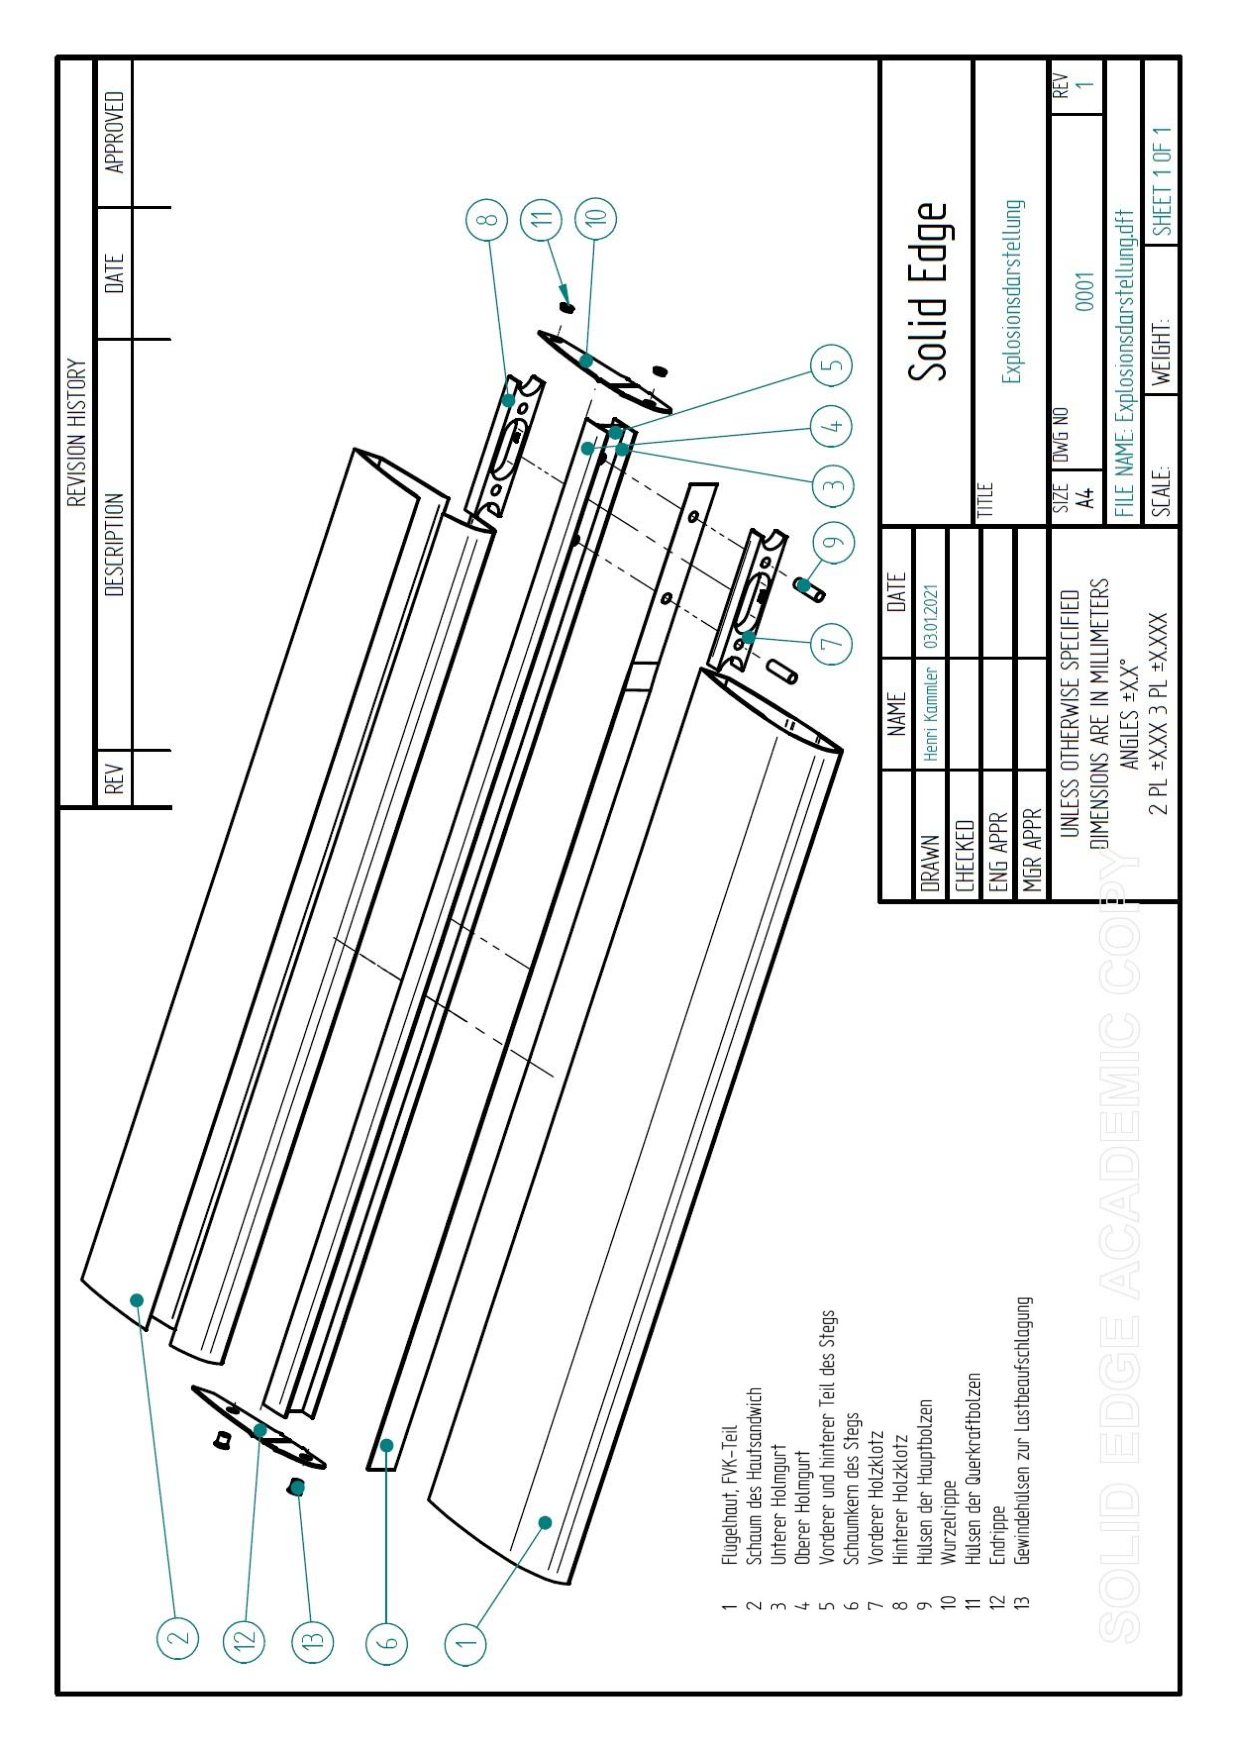
\includepdf[pages=-]{PDFs/ExplosionConvBez.pdf}
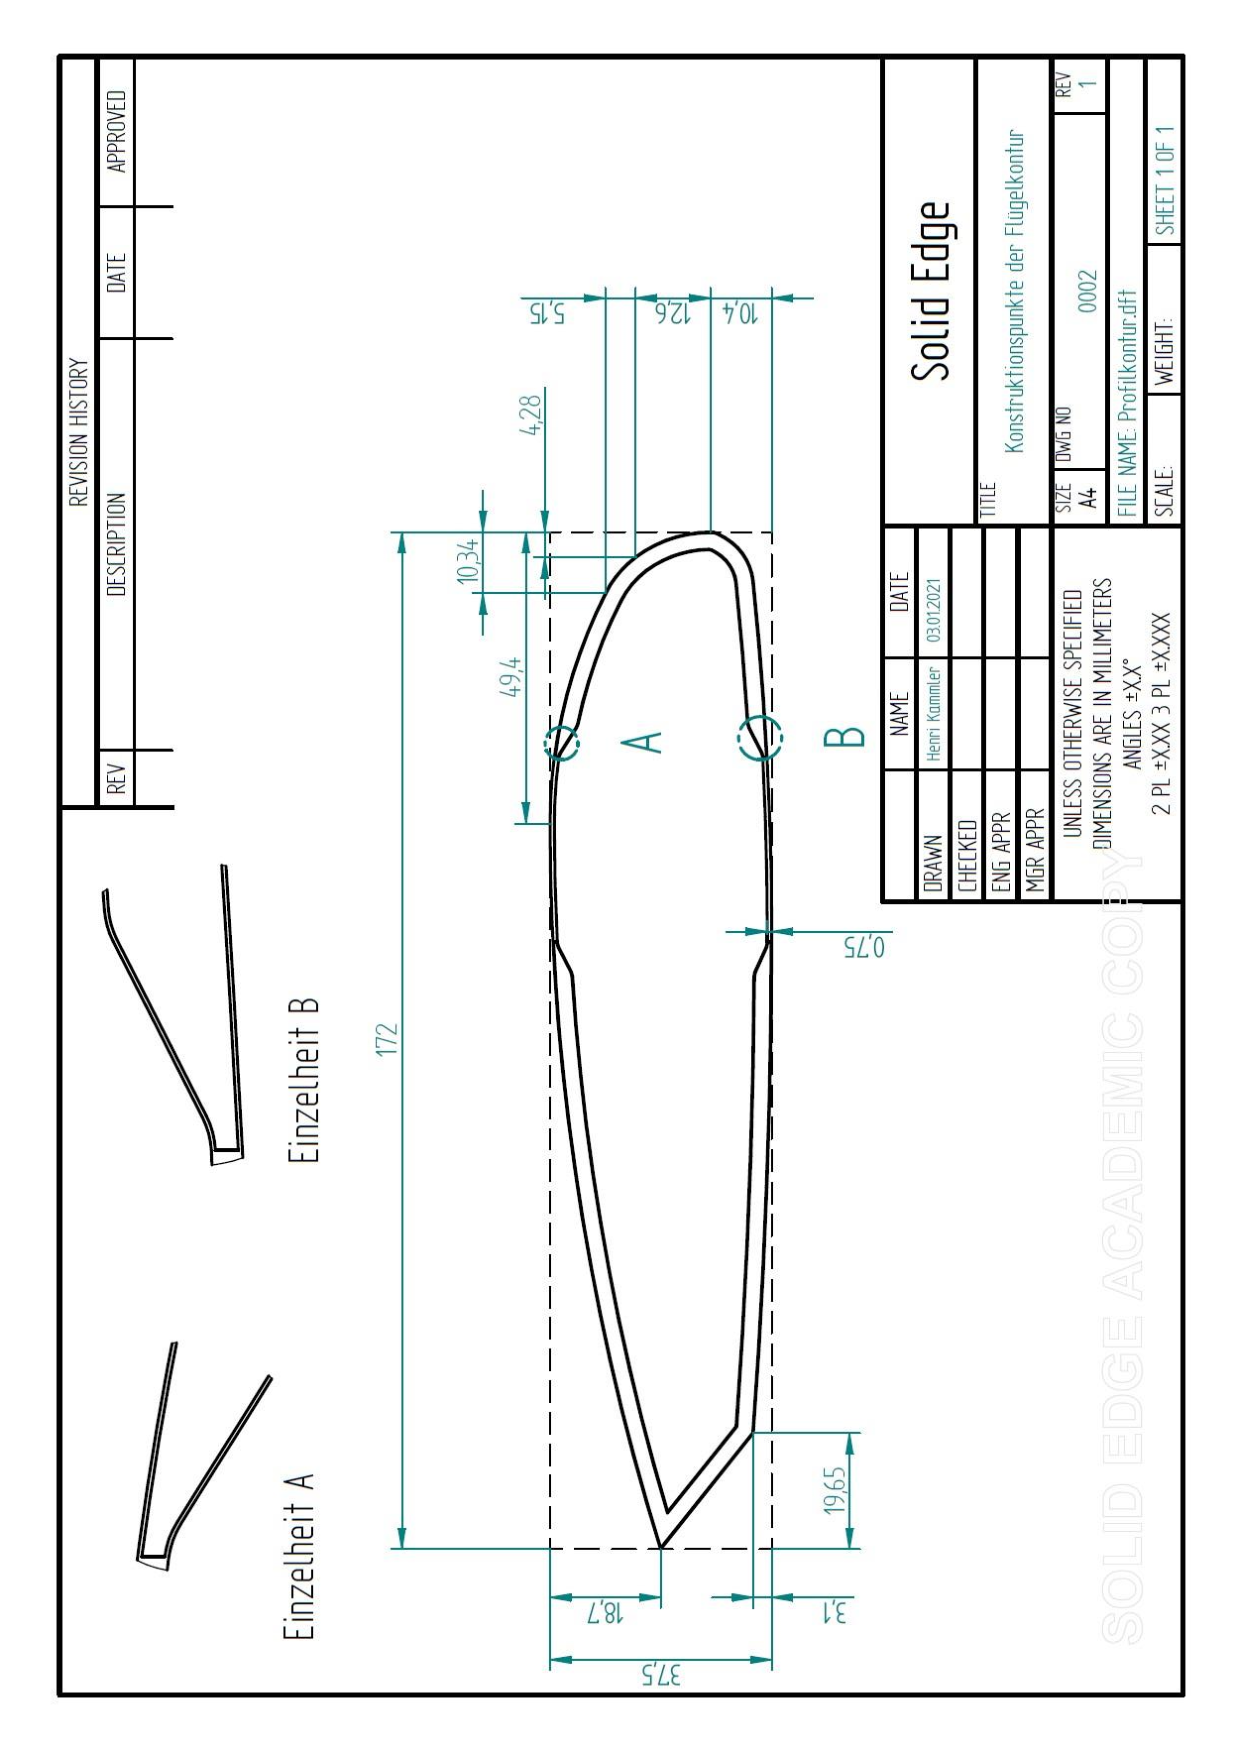
\includepdf[pages=-]{PDFs/ProfilkonturConv.pdf}
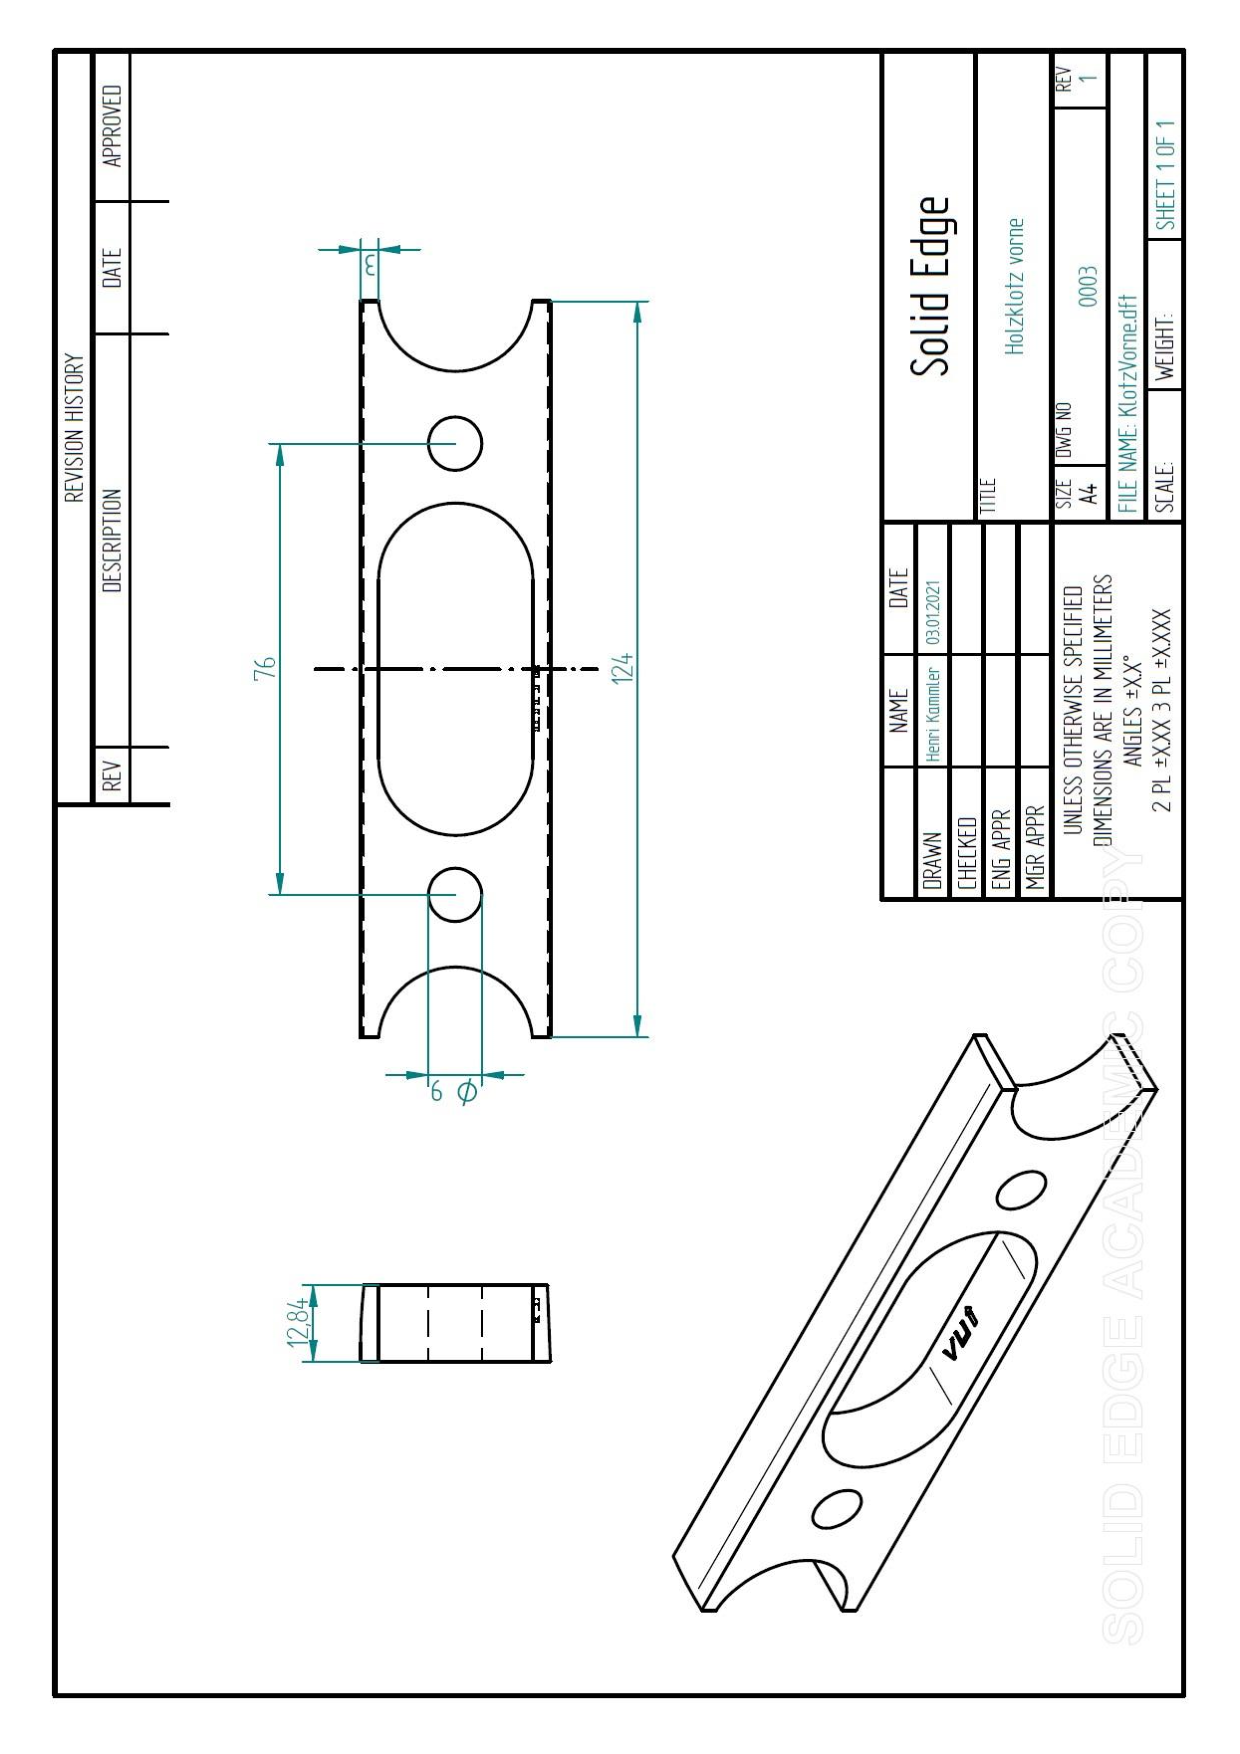
\includepdf[pages=-]{PDFs/KlotzVorne.pdf}
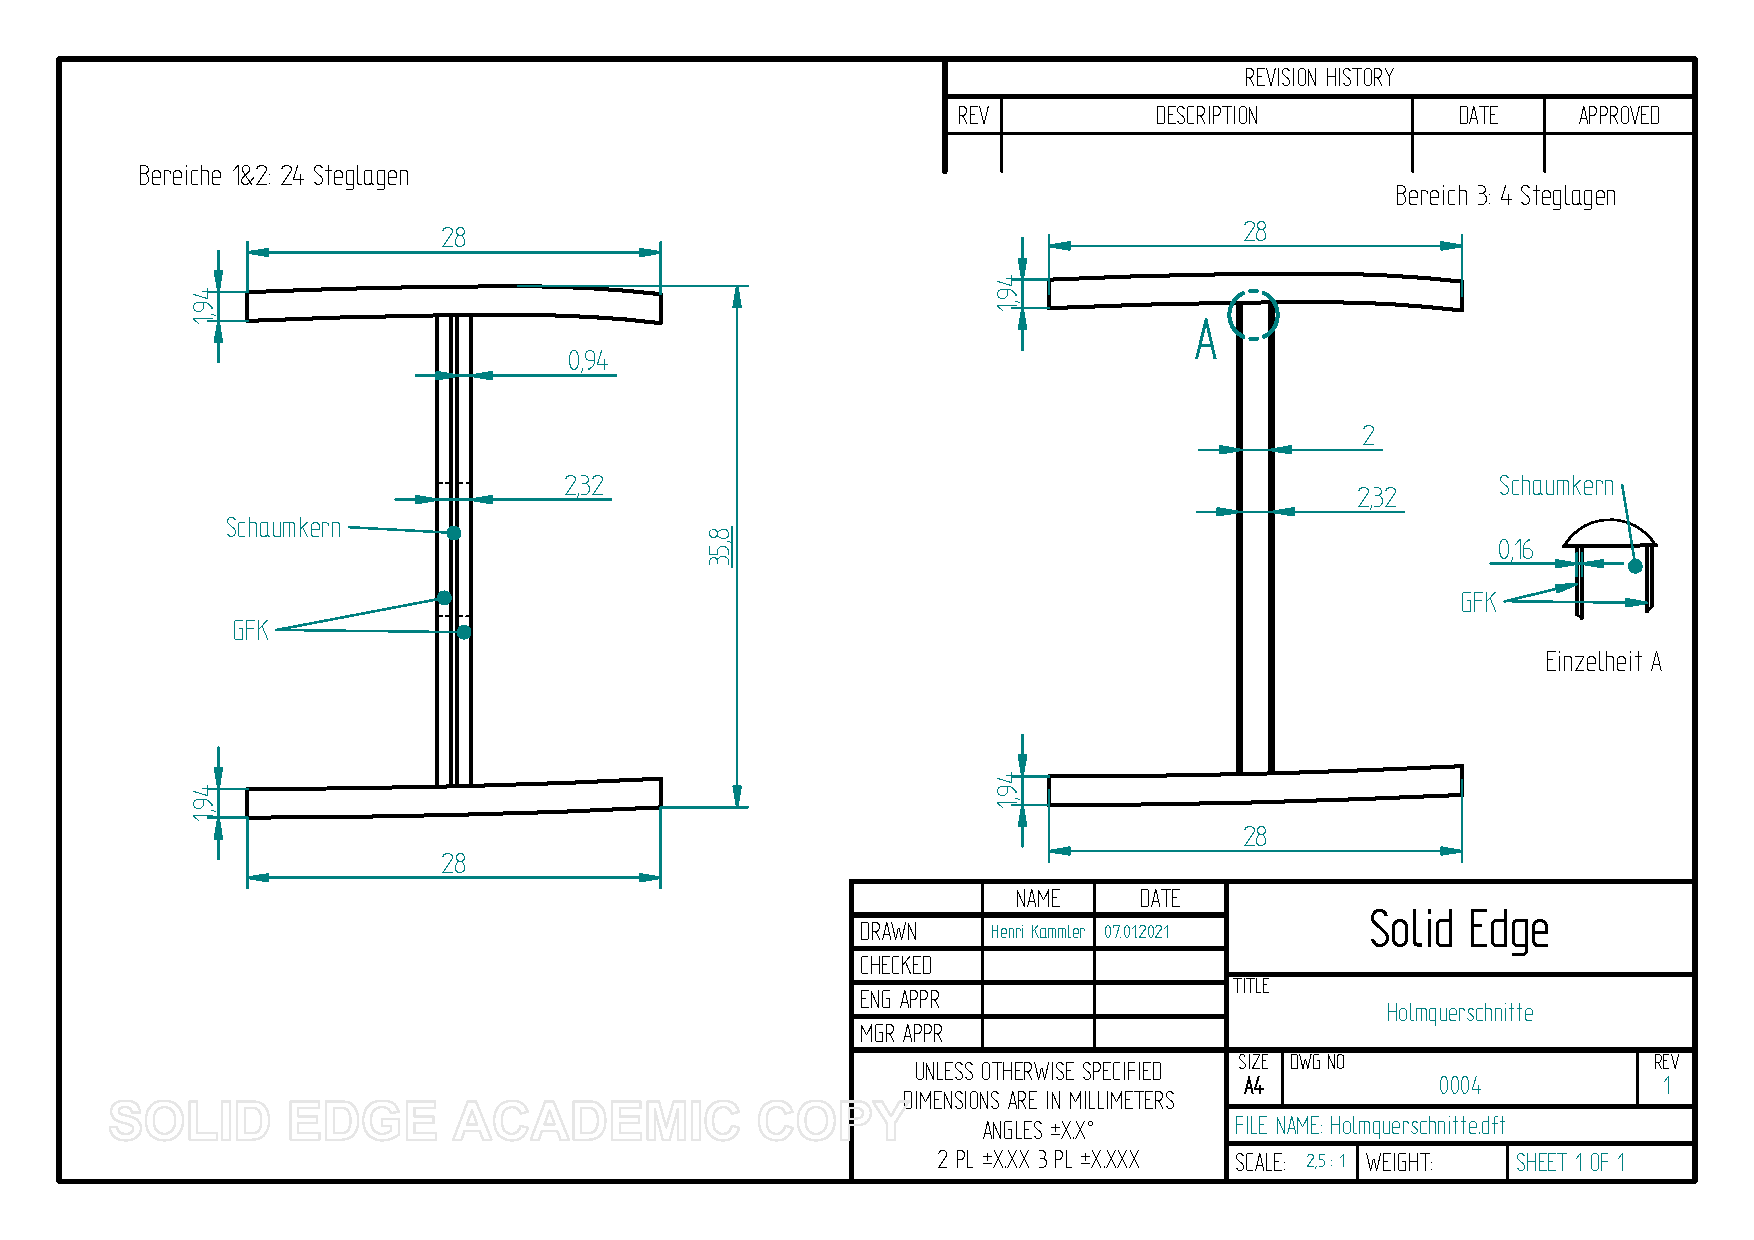
\includepdf[pages=-]{PDFs/Holmquerschnitte.pdf}

\begin{figure}[h]
	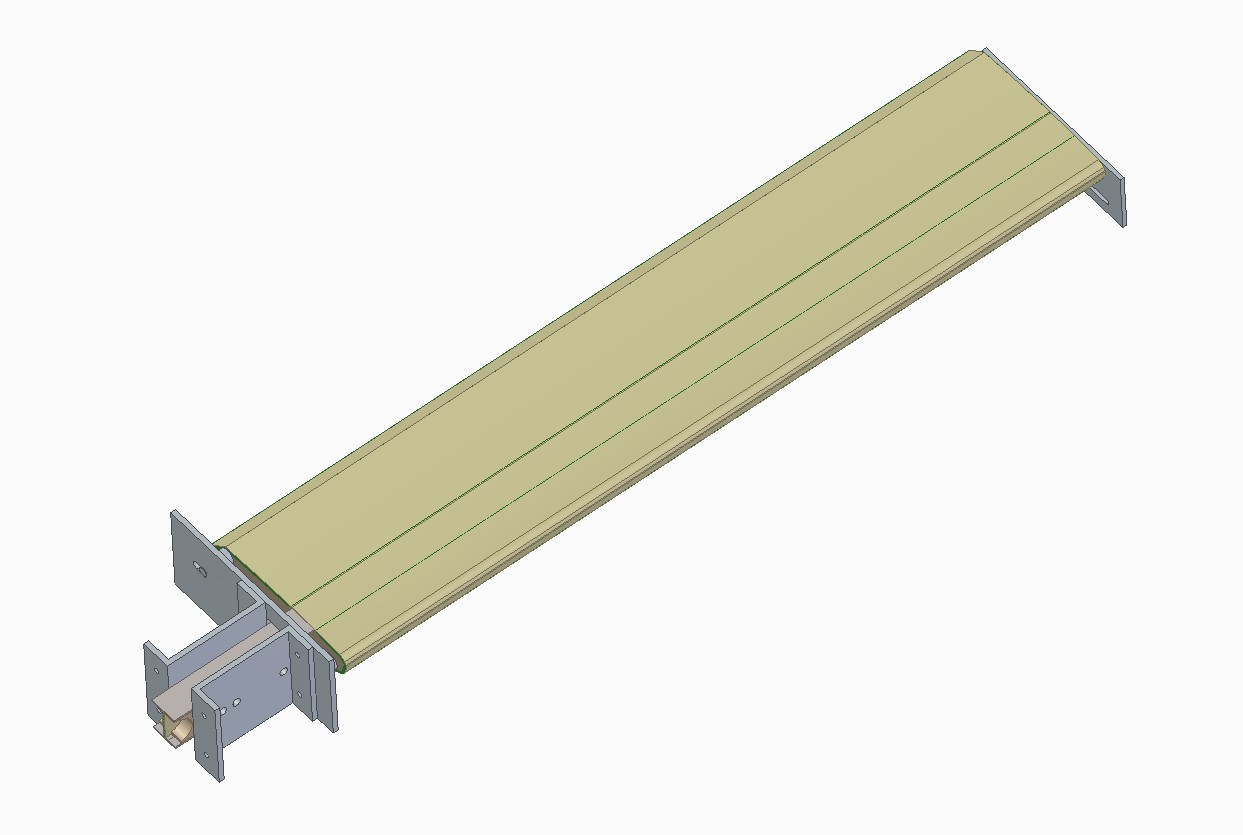
\includegraphics[width=1.0\textwidth]{Bilder/AufbauGesamt.jpg}
	\caption{CAD-Modell der Tragfläche und des Teststandes}
	\label{fig:AufbauGesamt}
\end{figure}

\begin{figure}[h]
	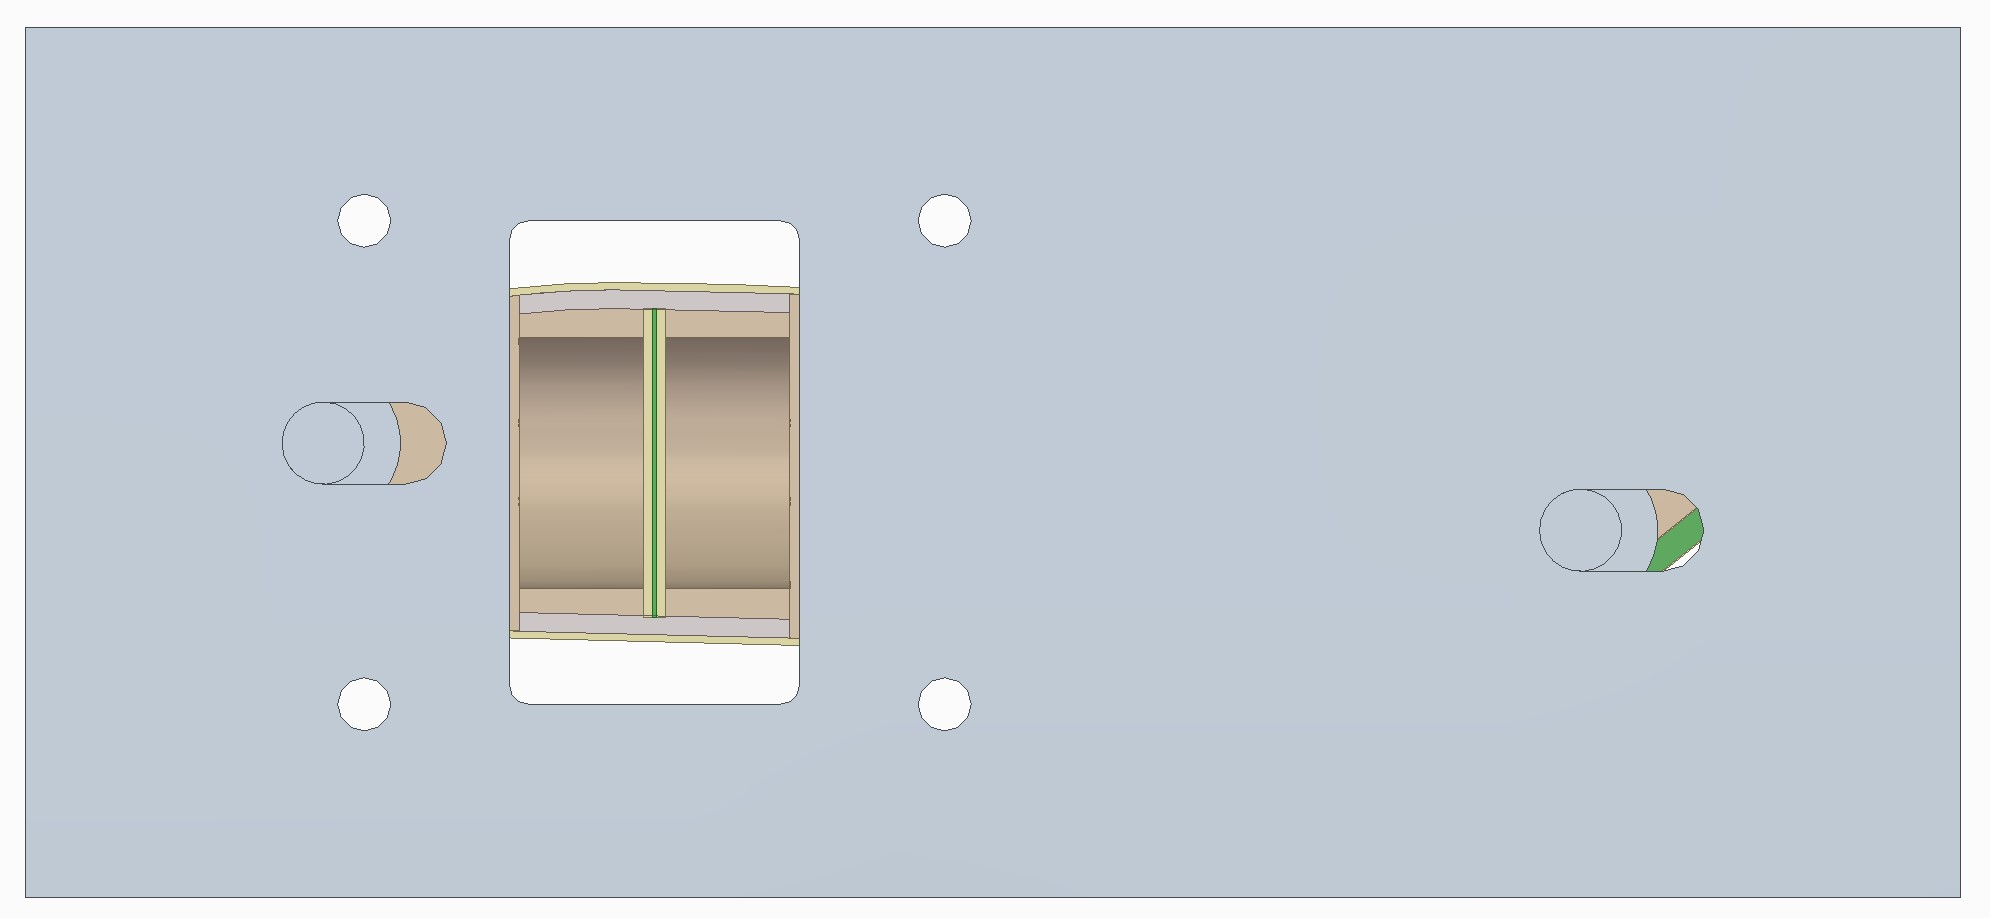
\includegraphics[width=1.0\textwidth]{Bilder/MontagePlatte.jpg}
	\caption{Montage der Tragfläche auf dem Teststand}
	\label{fig:MontagePlatte}
\end{figure}

